
\begin{figure}[t]
\centering
%\resizebox{\columnwidth}{%
\begin{tikzpicture}[x=1.2cm, y=1.2cm, font=\tiny,
  Component/.style={fill=white, draw, align=center, rounded corners=0.1cm, drop shadow={shadow xshift=0.05cm, shadow yshift=-0.05cm, fill=black}},
  Connection/.style={<->, >=stealth, shorten <=0.05cm, shorten >=0.05cm}]

\foreach \pos/\name in {1.6/pros3, 0.8/pros2} { %, 0.0/pros1} {
  \node [Component] (\name) at (\pos - 4, \pos) {Prosumer\\(\texttt{Python, geth})};
}

\node [Component] (dso) at (-1, 2.6) {DSO\\(\texttt{Python, geth})};

\node [Component] (solver) at (-4, 0) {Solver\\(\texttt{Python, CPLEX})};

\fill [fill=black!15] (90:1.5) -- (200:1.5) -- (340:1.5) -- (90:1.5);

\foreach \pos in {90, 200, 340} {
  \node [Component] at (\pos:1.5) {Blockchain\\ miner (\texttt{geth})};
}

\node [Component, dotted] (contract) at (0, 0) {Smart contract\\(\texttt{Solidity})};

%\draw [Connection, bend left=45] (solver) to (dso);

%\draw [Connection, bend left=65] (pros1) to node [midway, left, shift={(-0.25,0)}] {$\emptyset$MQ} (dso);
\draw [Connection, bend left=55] (pros2) to node [midway, left, shift={(-0.25,0)}] {$\emptyset$MQ} (dso);
\draw [Connection, bend left=45] (pros3) to (dso);

\draw [Connection, bend right=0] (solver) to node [midway, below left] {Ethereum} (contract);
\draw [Connection, bend right=15] (dso) to (contract);
%\draw [Connection, bend right=0] (pros1) to node [midway, below left] {Ethereum} (contract);
\draw [Connection, bend right=0] (pros2) to (contract);
\draw [Connection, bend right=0] (pros3) to (contract);
\end{tikzpicture}%
%}
\caption{Components of the energy trading system. In our implementation, we use Ethereum as the decentralized computation platform running smart contracts, and the other components interact with the blockchain network using the \texttt{geth} Ethereum client. The smart contract is implemented in Solidity, a high-level language for Ethereum, and it is executed by a network of \texttt{geth} mining nodes.}
\label{fig:components}
\end{figure}

\begin{figure*} [!t]
\centering
\begin{tikzpicture}[x=5.65cm, y=-0.063cm, semithick, font=\small,
RedDashed/.style={red, dashed}]
\def\posDSO{0}
\def\posProsumer{1}
\def\posLedger{2.05}
\def\posSolver{3}
\foreach \name/\pos in {DSO/\posDSO, Prosumer/\posProsumer, Smart contract/\posLedger, Solver/\posSolver} {
  \draw (\pos, 0) -- (\pos, 110);
  \node [draw, fill=white, rounded corners=0.1cm] at (\pos, 0) {\name};
}
\newcounter{seqTime}
\setcounter{seqTime}{0}
\foreach \action/\from/\to/\styl/\delta in {
  {withdrawAssets(anonAddress, energy, intervals, amount)/\posProsumer/\posDSO/solid/17},
  {failedWithdrawal(anonAddress, msg)/\posDSO/\posProsumer/red/8},
  {addEnergy(anonAddress, energy, intervals), addFinancialBalance(anonAddress, amount)/\posDSO/\posLedger/solid/14},
  {AssetAdded(anonAddress, energy, intervals)/\posLedger/\posProsumer/dashed/14},
  {postOffer({energy, intervals, price})/\posProsumer/\posLedger/solid/8},
  {OfferPosted({offerID, energy, intervals, price})/\posLedger/\posSolver/dashed/6},
%  {rescindOffer(offerID)/\posProsumer/\posLedger/red/6},
%  {OfferRescinded(offerID)/\posLedger/\posSolver/RedDashed/4},
  {submitSolution({powers, prices})/\posSolver/\posLedger/solid/8},
  {SolutionFinalized({powers, prices})/\posLedger/\posProsumer/dashed/6},
  {depositEnergy(energy, intervals), depositFinancial(amount)/\posProsumer/\posLedger/solid/14},
  {EnergyDeposited(anonAddress, energy, intervals), FinancialDeposited(anonAddress, amount)/\posLedger/\posDSO/dashed/14}%
} {
  \addtocounter{seqTime}{\delta}
  \draw [->, >=stealth, shorten <=0.05cm, shorten >=0.05cm, \styl] (\from, \value{seqTime}) -- (\to, \value{seqTime}) node [midway, above, align=center, text width={abs(\to - \from) * 5.1cm}, fill=white, fill opacity=0.67, text opacity=1] {\footnotesize\texttt{\scriptsize\action}};
}
\end{tikzpicture}
\caption{Sequence diagram of the trading workflow. Solid lines represent messages, including smart-contract function calls (i.e., blockchain transactions), while dashed lines represent smart-contract events. For ease of presentation, we show only a single prosumer and one instance of each communication. 
}
\label{fig:workflow}
\end{figure*}




\section{Energy Trading System}
\label{sec:tradingsystem}



In this section, we outline a system that can provide the energy trading and market clearing functionality described in the preceding sections. We first describe the main components of the system, including a short background on the runtime platform. 
Then, we give an overview of the messages exchanged between these components in the trading workflow. 





\subsection{Background}
% \begin{figure}
% 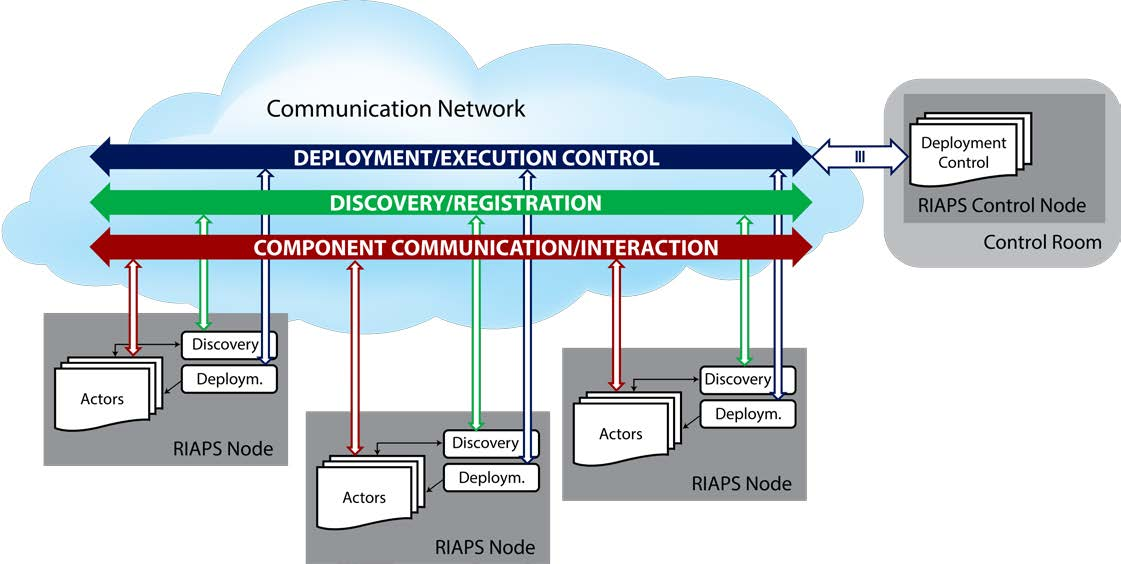
\includegraphics[width=0.48\textwidth]{diagrams/RIAPSBroch_FINALPRINT.jpg}
%   \caption{RIAPS concept.}
% 	\label{fig:concept}
% \end{figure}

In any technical system that relies on embedded computing, the most important ingredient is an ``operating system'' that provides the foundations for all algorithms, isolates the hardware details from the algorithms, and provides essential mechanisms for resource management, fault tolerance, and security. For example, in the work presented in this paper, this framework allows us to disseminate information between the actors. Our extended team has developed a platform called `Resilient Information Architecture Platform for Smart Grid' (RIAPS) \cite{riaps}, where each actor is a composition of several libraries that provide (1) a component model that provides a concurrent model of computation for building distributed real-time applications, (2) a messaging framework for facilitating interactions among actors, (3) a resource-management framework for controlling the use of computational resources, (4) a fault-management framework for detecting and mitigating faults in all layers of the system, (5) a security framework to protect the confidentiality, integrity, and availability of system under cyber-attacks, (6) a fault tolerant time synchronization service,  (7) a discovery framework for establishing the network of interacting actors of an application, and (7) a deployment and management framework for the administration and control of the distributed applications from a control room. 









\subsection{Trading System Architecture}
\label{sec:architecture}


Figure~\ref{fig:components} shows the architecture of the energy trading system. The specific platforms and tools used in our implementation are shown in parentheses and as arrow labels. All components are written in Python and communicate with each other using ZeroMQ, one of the protocols supported by the RIAPS platform. 




\subsection{Providing Privacy}
\label{sec:privacy}

To protect their privacy, prosumers use anonymous addresses when interacting with the blockchain (e.g., posting offers).
By generating new anonymous addresses at random periodically, they can prevent other participants from linking the anonymous addresses to their actual identities~\cite{Laszka17}, thereby keeping their trading activities private. 
However, in contrast with our prior work~\cite{Laszka17}, the addresses used in the workflow described in the next section are not completely anonymous. Since the blockchain-based smart contract has to check feeder-level safety constraints, each anonymous address must be linked to a feeder.
Hence, an anonymous address can hide only the prosumer's identity but not its feeder, which is a manifestation of the trade-off between safety and privacy.\footnote{Actually, participants can remain anonymous among a class of feeders with same number of participants and identical safety constraints.}

However, anonymous addresses pose a further threat to safety.
Since participants can generate anonymous addresses at almost no cost, they could post selling and buying offers for large amounts of energy, without any intention of delivering and without facing any repercussions.
A malicious or faulty participant could easily destabilize the grid with this form of reckless trading.
Consequently, the amount of energy that may be traded by anonymous addresses belonging to a participant must be limited.

Thus, we use the concept of energy assets, initially introduced  in~\cite{Laszka17} and  used in the trading workflow described in the next section.
%\AronC{They were only used but not described in the workflow.}  described in the workflow of above.
%In~\cite{Laszka17}, we introduced \emph{energy assets} to enforce participant-level safety constraints.
An energy asset represents a permission to sell or buy a specific amount of energy in a specific set of  time intervals. 
Each prosumer can ask the DSO to transfer assets to an anonymous address, who can check whether it would be safe to give permission to the participant.
If it would be, then the DSO records this transfer on the blockchain.
Later, when the participant posts an offer from the anonymous address, the smart contract can check whether the address has the assets required for the offer.
Since only the DSO can link the anonymous address to the participant, assets enable enforcing participant-level constraints without violating privacy.


\subsection{Trading Workflow}

Figure~\ref{fig:workflow} illustrates the trading workflow.
For ease of presentation, the figure shows only one prosumer and only a single message of each type.
In practice, a large number of prosumers may interact with the DSO and the smart contract, and each of them may exchange multiple messages.

\newcommand{\msgDesc}[1]{{\footnotesize{\texttt{#1}}}}

The workflow includes the following messages:
\begin{compactitem}
\item 
\msgDesc{withdrawAssets(anonAddress, energy, intervals, amount)}: message sent by a prosumer to the DSO, asking the DSO to transfer energy and/or financial assets from the prosumer's account at the DSO to an anonymous address.
Before sending this message, the prosumer first generates a random anonymous address to protect her privacy.
The message specifies the assets that the prosumer wishes to withdraw (i.e., amount of energy and time intervals) and the anonymous address to which the DSO should transfer them.
Note that the prosumer may send this message long before actually engaging in trading, so the DSO does not have to be online continuously.
\item \msgDesc{failedWithdrawal(anonAddress, msg)}: message sent by the DSO to the prosumer,
notifying the prosumer that the requested assets cannot be withdrawn due to, e.g., energy safety requirements or insufficient funds.
\item \msgDesc{addEnergy(anonAddress, energy, intervals)},\\\msgDesc{addFinancialBalance(anonAddress, amount)}:
smart contract functions called by the DSO (i.e., transactions recorded on the blockchain) in response to the prosumer's request, creating energy and financial assets on the blockchain and transferring them to an anonymous address.
Before recording this transaction, the DSO must first verify that enabling the prosumer to trade these assets does not violate any safety constraints and that the anonymous address is linked to the correct feeder.
%The call specifies the assets and the anonymous address to which they are transferred. 
\item \msgDesc{AssetAdded(anonAddress, energy, intervals)},\\\msgDesc{FinancialAdded(anonAddress, amount)}: broadcast messages emitted by the smart contract (i.e., events logged on the blockchain),
notifying the prosumer that the requested assets have been transferred to the anonymous address.
\item \msgDesc{postOffer(energy, intervals, price)}: smart-contract function called by a prosumer (from its anonymous address), publicly posting an energy bid or ask.
%If the prosumer is interested in buying energy, then it posts an energy bid, which specifies an energy consumption asset and a price.
%If the prosumer is interested in selling, then it posts an energy ask, which specifies an energy production asset and a price.
%In both cases, the transaction must be cryptographically signed by the private key of the address, and it locks the assets until the offer is accepted or rescinded.
\item \msgDesc{OfferPosted(offerID, energy, intervals, price)}:
message broadcast by the smart contract, notifying solvers that an offer was posted.
\item \msgDesc{submitSolution(powers, prices)}:
smart-contract function called by a solver,
submitting a new solution for the energy trading problem. %If the offer was an energy bid, then the other prosumer has to provide an energy production assets;
%if the offer was an energy ask, then the other prosumer has to provide both energy consumption and financial assets.
%In both cases, the transaction must be cryptographically signed by the private key of the other prosumer's anonymous address.
%If there is an overlap between the time intervals of the offered asset, and the asset provided by the other prosumer, then the intersecting parts of the assets are exchanged and the non-overlapping parts are returned to their original owners.
%Similarly, based on the price and exchanged energy assets, a part of the financial asset is transferred to the seller, while the rest is returned to the seller. 
\item \msgDesc{SolutionFinalized(powers, prices)}:
message broadcast by the smart contract,
notifying both prosumers and solvers of energy trades that have been finalized. %that its offer has been accepted, and the assets have been exchanged.
\item \msgDesc{depositEnergy(energy, intervals)},\\\msgDesc{depositFinancial(amount)}:
smart-contract functions called by a prosumer,
depositing energy and financial assets to the prosumer's account.
%The transaction specifies the assets, and it must be cryptographically signed by the anonymous address that owns them.
Note that to protect privacy, the calls do not specify the prosumer, so the DSO has to keep track of which prosumer has used which anonymous address.
\item \msgDesc{EnergyDeposited(anonAddress, energy, intervals)},\\\msgDesc{FinancialDeposited(anonAddress, amount)}:
messages broadcast by the smart contract,
notifying the DSO that assets have been deposited from anonymous address, which triggers the transfer of these assets to the prosumer's account at the DSO.
\end{compactitem}

\subsection{Implementation Considerations}
\label{sec:implementation}

\subsubsection{Parameters} The system of prosumers, solvers, DSO, and smart contract operates mostly asynchronously. The only synchronous communication  occurs between prosumers and the DSO. They all operate as  independent processes running on remote nodes, with their own time bases. In particular, the solver can operate as a periodic process (with a period $\Delta_s$), waiting on information from the smart contract about all the offers that have been posted in the prior period. The prosumers  can also operate as periodic processes, submitting their offers and bids to the smart contract.  In practice, prosumers will be synchronized with real wall-clock time, making their bids and asks known for future intervals, depending upon the time at which they post their bids/asks and how far in the future  they can predict their usage or operation. We make  their prediction window $L$ a parameter of the system. The value of this parameter is at least $2$, because prosumers have to  make a bid/ask for at least the next interval (we count the current interval in $L$). A larger value of this prediction window will increase the risk of uncertainty for the prosumer, since they are expected to be able to fulfill their bid or ask.\footnote{The size of the prediction window is part of the prosumer strategy, which is not explored in this paper as our focus is on the implementation of the TMP.} Additionally, during our experiments, we can simulate $\Delta$ as $\hat{\Delta}$ to speed up the process.\footnote{Note that this is the amount of real time passed in the simulation before proceeding to the next interval. This allows us to speed things up for the experiment, since running the system slower would just be easier.} These parameters are described in Table \ref{tab:symbols}.

\subsubsection{Speed and Synchronization Considerations}
A relevant problem for TMP is deciding how fast it can run and ensuring that trades for the next interval can clear before the $T_{clear}$ parameter, which has a minimum bound of $1$.
In our system, regular network communication mechanisms are assumed to be fast. However, the communication with the smart contract is limited by the block mining rate, and we need multiple messages exchanged in each interval (see Figure~\ref{fig:workflow}), so the miners need to work fast enough to mine a few blocks in each time interval. In a closed environment, this can be achieved by reducing the difficulty of the cryptographic puzzle solved for proof-of-work consensus. In our system, as shown in the next section, we are able to clear transactions much faster than one time interval. 
For larger systems, the proof-of-work consensus may be replaced by, e.g., proof-of-stake, for scalability.

Another problem is the synchronization between the different agents. The runtime platform of RIAPS provides us with high-precision time synchronization \cite{riaps2}. However, even if we only have NTP as the synchronization mechanism, we can operate the system correctly. This is because intervals in practice are relatively (i.e.,  compared to typical communication delays) long (e.g., 15 minutes). Additionally, the smart contract can ensure that the system always proceeds to the next time interval (however, the accuracy of this is limited by the mining rate, see previous paragraph). Additionally, our system can  tolerate or discard out-of-order and late messages due to the event chronology implemented in the blockchain platform. In practice, however, prosumers should try to post their offers early within a time interval, so that solvers will include them in the solution for the current time interval. On the other hand, solvers should wait some time before starting to work, so that they can collect all (or at least most) of the offers posted in the interval.

% \Aron{Talk about timing issues in smart contracts!}

% \color{red}
% Ideas:
% \begin{itemize}
% \item communication over the blockchain is limited by the block mining rate, and we need multiple messages exchanged in each interval, so the miners need to work fast enough to mine a few blocks in each time interval
% \item no time synchronization is necessary since 1) intervals in practice are relatively (i.e.,  compared to typical communication delays) long (e.g., 15 minutes) 2) smart contract can ensure that the system always proceeds to the next time interval (however, the accuracy of this is also limited by the mining rate, see previous point) 3) our system can tolerate or discard out-of-order and late messages\AbhishekC{Can we address what will happen if there are multiple miners.}
% \item in practice, prosumers should try to post their offers early within a time interval, so the solver can include them in the solution for the current time interval; on the other hand, solvers should wait some time before starting to work so that they have all (or at least most) of the offers posted in the interval
% \end{itemize}
% \color{black}
